\section{Vorlesung 04.05.2016}

\subsection{Vertebraten:}\footnote{\url{https://de.wikipedia.org/wiki/Wirbeltiere}} Wirbeltiere (Vertebrata) sind Tiere, die eine Wirbelsäule besitzen. Zu den Vertebraten gehören fünf klassische Großgruppen: Säugetiere, Vögel, Reptilien, Amphibien sowie Fische (Knochen- und Knorpelfische), als urtümliche Vertreter zudem die Rundmäuler.

\subsection{Invertebraten:}\footnote{\url{https://de.wikipedia.org/wiki/Wirbellose}} Wirbellose, Invertebrata oder Evertebrata sind vielzellige Tiere ohne Wirbelsäule. Zu dieser informellen Gruppe (Formtaxon) von Lebewesen gehört die Mehrzahl aller bekannten Tierarten.

\subsection{Nervenzelle:}\footnote{\url{https://de.wikipedia.org/wiki/Nervenzelle}} Eine Nervenzelle oder ein Neuron ist eine auf Erregungsleitung und Erregungsübertragung spezialisierte Zelle, die als Zelltyp in Gewebetieren und damit in nahezu allen vielzelligen Tieren vorkommt. Die Gesamtheit aller Nervenzellen eines Tieres bildet zusammen mit den Gliazellen das Nervensystem.\\
Eine typische Säugetier-Nervenzelle hat einen Zellkörper und Zellfortsätze zweierlei Art: die Dendriten und den Neuriten bzw. das Axon. Die verästelten Dendriten nehmen vornehmlich Erregung von anderen Zellen auf. Der Neurit eines Neurons, von Gliazellen umhüllt sein Axon, kann über einen Meter lang sein und dient zunächst der Fortleitung einer Erregung dieser Zelle in die Nähe anderer Zellen. Dabei wird eine Spannungsänderung über den Fortsatz weitergeleitet, indem kurzzeitige Ionenströme durch besondere Kanäle in der Zellmembran zugelassen werden.
Die Axonenden stehen über Synapsen, an denen die Erregung selten unmittelbar elektrisch weitergegeben, sondern meist mittels Botenstoffen (Neurotransmittern) chemisch übertragen wird, in Kontakt zu anderen Nervenzellen, Muskelzellen (neuromuskuläre Endplatte) oder zu Drüsenzellen.

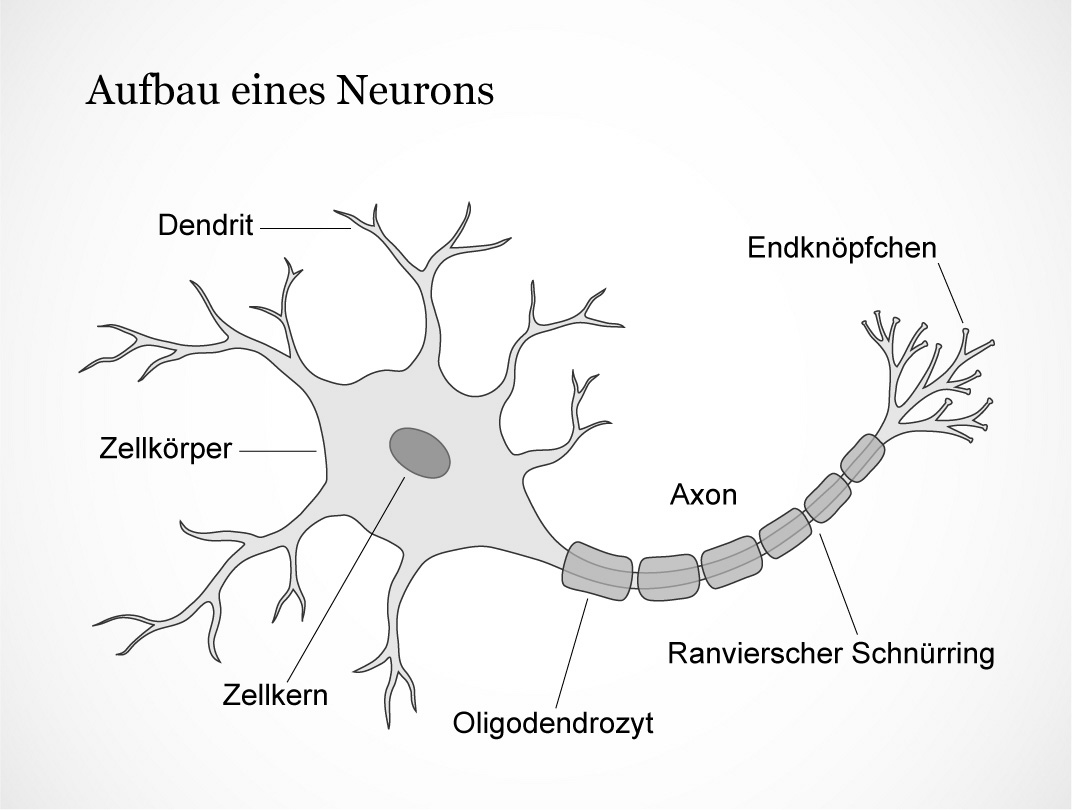
\includegraphics[width=0.6\textwidth]{lectures/160405/pix/neuron.jpg}

\subsection{Axon:}\footnote{\url{https://de.wikipedia.org/wiki/Axon}} Das Axon, selten der Axon, auch Neuraxon oder Achsenzylinder genannt, ist ein oft langer schlauchartiger Nervenzellfortsatz, ein Neurit, der in einer Hülle von Gliazellen verläuft und zusammen mit dieser Umhüllung als Nervenfaser bezeichnet wird. Seitliche Abzweigungen des Axons werden auch dessen Kollaterale genannt und können sich wie das terminale Axon in mehrere Endästchen aufzweigen. Die meisten Neuronen haben ein einziges Axon. Es gibt aber auch Nervenzellen, die kein Axon besitzen, z. B. verschiedene Amakrinzellen der Netzhaut.

\subsection{Dendriten:}\footnote{\url{https://de.wikipedia.org/wiki/Dendrit_\%28Biologie\%29}} Dendriten heißen in der Biologie Zellfortsätze von Nervenzellen, die aus dem Zellkörper hervorgehen und vorwiegend der Reizaufnahme dienen. Eine Nervenzelle besteht typischerweise aus drei Anteilen: dem Zellkörper, Soma oder Perikaryon genannt, und Zellfortsätzen, die Dendriten einerseits und der Neurit – in Gliahülle das Axon – andererseits. Es gibt auch spezialisierte Neuronen, die kein Axon haben (z. B. die Amakrinzellen der Netzhaut) oder die keine Dendriten besitzen (z. B. die Stäbchen und Zapfen der Netzhaut) oder solche, bei denen der Zellkörper nicht mehr zwischen Dendritenstamm und Axon liegt und die Fortsätze so ineinander übergehen (pseudouniploare wie bei den sensiblen Spinalganglienzellen).
\\
Nervenzellen werden morphologisch nach der Anzahl ihrer Fortsätze unterschieden:
1: unipolare Nervenzelle, 2: bipolare Nervenzelle, 3: multipolare Nervenzelle, 4: pseudounipolare Nervenzelle\\
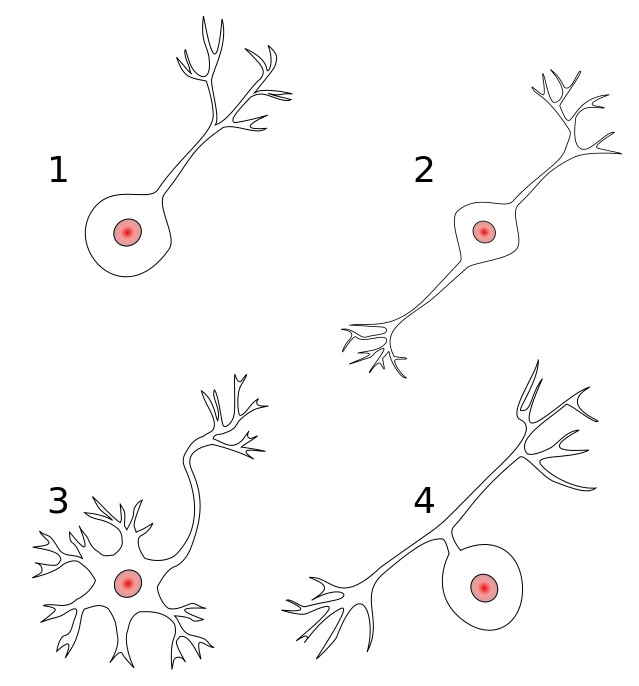
\includegraphics[width=0.6\textwidth]{lectures/160405/pix/dendrite.jpg}

\subsection{Synapse:}\footnote{\url{https://de.wikipedia.org/wiki/Synapse}} Synapse bezeichnet die Stelle einer neuronalen Verknüpfung, über die eine Nervenzelle in Kontakt zu einer anderen Zelle steht – einer Sinneszelle, Muskelzelle, Drüsenzelle oder anderen Nervenzellen. Synapsen dienen der Übertragung von Erregung, erlauben aber auch die Modulation der Signalübertragung, und sie vermögen darüber hinaus durch anpassende Veränderungen Information zu speichern. Die Anzahl der Synapsen beträgt im Gehirn eines Erwachsenen etwa 100 Billionen (1014) – bezogen auf ein einzelnes Neuron schwankt sie zwischen 1 und 200.000.

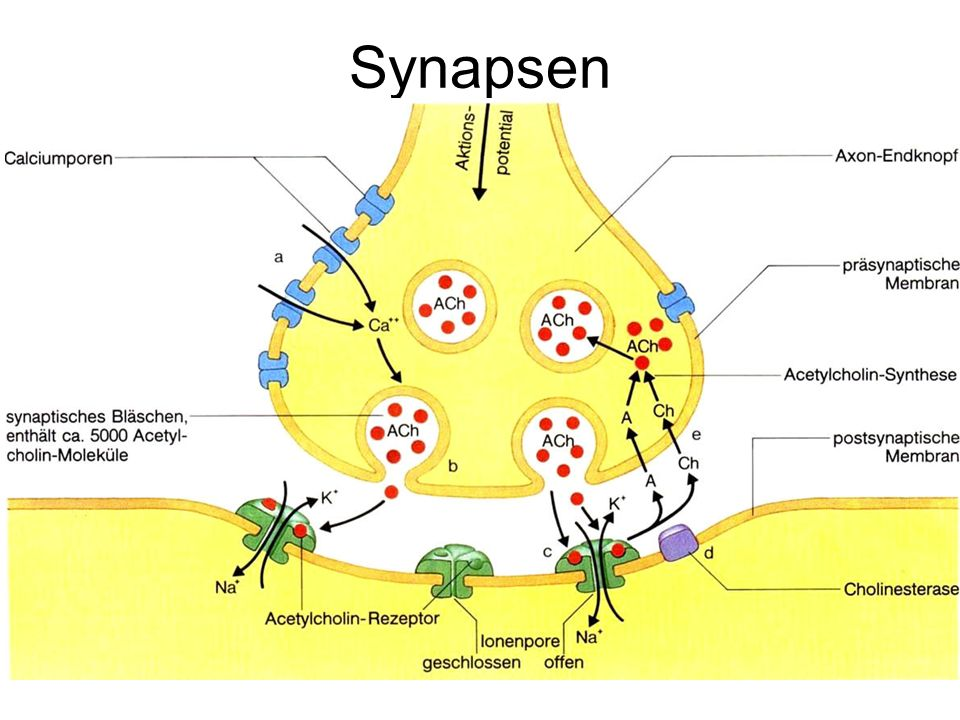
\includegraphics[width=0.95\textwidth]{lectures/160405/pix/synapse.jpg}
In den meisten Fällen sind es chemische Synapsen. Bei ihnen wird das Signal, das als elektrisches Aktionspotential ankommt, in ein chemisches Signal umgewandelt, in dieser Form über den zwischen den Zellen bestehenden synaptischen Spalt getragen, und dann wieder in ein elektrisches Signal umgebildet. Dabei schüttet die sendende Zelle (präsynaptisch) Botenstoffe aus, Neurotransmitter, die sich auf der anderen Seite des Spaltes (postsynaptisch) an Membranrezeptoren der empfangenden Zelle binden. Hierdurch ist die Richtung der Signalübertragung (nur vorwärts) anatomisch festgelegt, was für die Verarbeitung von Information in neuronalen Netzen grundlegend ist. Der erregungsübertragende Transmitter wird entweder in der Endigung des Axons des sendenden Neurons gebildet oder in dessen Zellkörper synthetisiert und axonal zu den präsynaptischen Membranregionen transportiert.
Dagegen sind elektrische Synapsen als gap junctions Kontaktstellen, bei denen Ionenkanäle zweier Zellen unmittelbar aneinander koppeln und so einen Übergang von Ionen und kleinen Molekülen von einer Zelle zur anderen erlauben. Zuerst wurden solche Synapsen zwischen Neuronen entdeckt, doch kommen ähnliche Kontaktstellen noch in anderen Geweben vor, auch in Pflanzen.
In übertragenem Sinn werden als immunologische Synapsen die Stellen vorübergehender zellulärer Kontakte von Zellen des Immunsystems bezeichnet, sowohl untereinander als auch mit Zellen des umgebenden Gewebes. Dabei binden Moleküle auf der Oberfläche der einen Zelle an Rezeptormoleküle und Adhäsionsmoleküle in der Zellmembran der anderen und tauschen darüber Informationen aus.

\subsection{Vesikel:}\footnote{\url{https://de.wikipedia.org/wiki/Vesikel_\%28Biologie\%29}} Vesikel (lat. vesicula - Bläschen) in der Biologie sind intrazelluläre (in der Zelle gelegene), sehr kleine, rundliche bis ovale Bläschen, die von einer einfachen oder doppelten Membran oder einer netzartigen Hülle aus Proteinen umgeben sind. Die Vesikel bilden eigene Zellkompartimente, in denen unterschiedliche zelluläre Prozesse ablaufen. Ihre Größe beträgt etwa ein Mikrometer. Vesikel sind für den Transport vieler Stoffe in der Zelle verantwortlich.

\subsection{Gliazelle:}\footnote{\url{https://de.wikipedia.org/wiki/Gliazelle}} Gliazelle ist ein Sammelbegriff für strukturell und funktionell von den Nervenzellen (Neuronen) abgrenzbare Zellen im Nervengewebe. Nach heutigen Erkenntnissen bilden Gliazellen nicht nur ein Stützgerüst für Nervenzellen, sondern sorgen auch durch ihre Umhüllung für deren elektrische Isolation. Weiterhin sind Gliazellen maßgeblich an Stofftransport und Flüssigkeitsaustausch sowie an der Aufrechterhaltung der Homöostase im Gehirn beteiligt. Darüber hinaus wirken sie auch im Prozess der Informationsverarbeitung, -speicherung und -weiterleitung mit.
Etwa die Hälfte der Zellen im menschlichen Gehirn sind Gliazellen, ähnlich wie bei anderen Primaten. Gliazellen sind meist kleiner als die Nervenzellen, im Unterschied zu diesen variiert ihre durchschnittliche Zellmasse im Nervengewebe nur gering bei verschiedenen Säugetierspezies. In deren Hirnstrukturen hängt das jeweilige Verhältnis von Glia zu Neuronen nach Anzahl und Volumen hauptsächlich von der durchschnittlichen Neuronengröße ab.

\subsection{Myelinisierung:}\footnote{\url{https://de.wikipedia.org/wiki/Nervenfaser}} Myelinisierung wird die mehrfache Umwicklung des Neuriten einer Nervenzelle durch umhüllende Gliazellen genannt, wodurch das Axon elektrisch derart isoliert wird, dass mit Umbau seiner Internodien eine schnellere Erregungsleitung möglich wird.

\subsection{Neurotransmitter:}\footnote{\url{https://de.wikipedia.org/wiki/Neurotransmitter}} Neurotransmitter sind Botenstoffe, die an chemischen Synapsen die Erregung von einer Nervenzelle auf andere Zellen übertragen (synaptische Transmission). Die Neurotransmitter werden im Zellkörper oder in der Endigung des Axons vom sendenden Neuron synthetisiert und in Quanten freigesetzt.

\subsection{Aktionspotential:}\footnote{\url{https://de.wikipedia.org/wiki/Aktionspotential}}Aktionspotential oder elektrische Erregung ist eine vorübergehende charakteristische Abweichung des Membranpotentials einer Zelle von ihrem Ruhepotential.
\\\\
\textbf{Grundlage}\\
Ein Aktionspotential kann von etwa einer Millisekunde bis zu einigen Minuten dauern. Es gibt keine starken oder schwachen Aktionspotenziale, vielmehr sind es Alles-oder-Nichts-Reaktionen. Sie entstehen typischerweise am Axonhügel einer Nervenzelle und wandern das Axon entlang. Die Signalstärke wird in der Frequenz von Aktionspotenzialen wiedergegeben. Aktionspotentiale breiten sich auch rückwärts über den Zellkörper und die Dendriten aus. Die Funktion dieser Weiterleitung wird noch untersucht. Axonale Ausbreitung vom Zellkörper zum Endknöpfchen wird auch orthodrom (richtig) genannt und die gegenläufige Weiterleitung antidrom.

Die Ursachen für die Ausbildung und die besonderen Eigenschaften eines Aktionspotentials liegen in den Eigenschaften verschiedener Gruppen von Ionenkanälen in der Plasmamembran der Zelle. Ein anfänglicher Reiz aktiviert, sobald er eine bestimmte Schwelle erreicht (ca. -50 mV; sog. Schwellenpotential), und ohne Rücksicht darauf, wie weit er sie übersteigt, eine Kette von Öffnungs- und Schließungsvorgängen der Kanäle, die einen Ionenstrom ermöglichen und damit das Membranpotential verändern. Die Form des Aktionspotentials ist dann, unabhängig von der Stärke des auslösenden überschwelligen Reizes, immer gleichförmig. Diese Änderung des Potentials kann an der nächsten Stelle der Membran wieder eine elektrische Erregung bewirken, was die Grundlage der Erregungsleitung ist.
\\\\
\textbf{Potentialverlauf}\\
Ausgehend vom Ruhemembranpotential, das bei Neuronen je nach Zelltyp zwischen -90 und -70 mV liegt, werden vier Phasen des Aktionspotentials unterschieden:
\begin{enumerate}
	\item In der Initiationsphase treibt ein Reiz die negative Spannung in Richtung null (Depolarisation). Dies kann langsam oder schnell geschehen und ist unterhalb des Schwellenpotentials umkehrbar. Solch ein Reiz kann ein sich räumlich näherndes Aktionspotential sein oder ein postsynaptischer Ionenstrom.
	\item Falls das Schwellenpotenzial überschritten wird, beschleunigt sich die Depolarisation stark (Aufstrich). Das Membranpotenzial wird sogar positiv (Overshoot).
	\item Auf das Maximum bei +20 bis +30 mV folgt die Rückkehr in Richtung Ruhepotential (Repolarisation).
	\item In vielen Neuronen wird das Ruhepotenzial zunächst unterschritten, bis z.B. -90 mV, und schließlich von negativeren Werten her erreicht. Dies wird als Hyperpolarisation oder hyperpolarisierendes Nachpotential bezeichnet. Während der Hyperpolarisation kann noch kein weiteres Aktionspotential ausgelöst werden, woraus sich die Maximalfrequenz von Aktionspotentialfeuer ergibt (der Begriff Feuern wird auch in wissenschaftlicher Literatur für das Generieren von Aktionspotentialen benutzt).
\end{enumerate}

Ein Aktionspotential dauert etwa 1–2 ms in Neuronen, kann sich aber auch über einige hundert Millisekunden (im Herzen) erstrecken.

Bereits während der Repolarisation befindet sich die Zelle in der Refraktärphase. Während dieser Phase kann zunächst kein (absolute Refraktärzeit, ca. 0,5 ms) und danach nur mit erhöhtem Reiz (erhöhtes Schwellenpotential innerhalb der relativen Refraktärzeit, ca. 3,5 ms) ein weiteres Aktionspotential erzeugt werden.

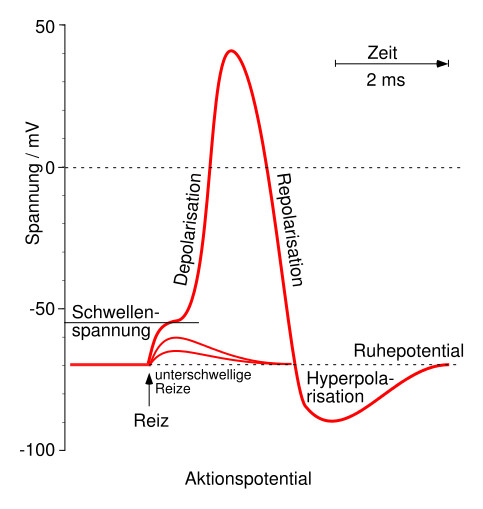
\includegraphics[width=0.7\textwidth]{lectures/160405/pix/Aktionspotential.jpg}

\textbf{Urachen}\\
Die Erklärung setzt das Verständnis der im Artikel zum Ruhemembranpotential vorgestellten Entstehung eines Ruhemembranpotentials voraus. Kurz zusammengefasst sind folgende Faktoren für das Ruhemembranpotential verantwortlich:
\begin{itemize}
    \item chemische- und elektrische Gradienten von Ionen
    \item Selektive Permeabilität von Ionenkanälen
    \item Ionenpumpen – insbesondere Natrium-Kalium-Pumpen.
\end{itemize}

\subsection{Exozytose}\footnote{\url{https://de.wikipedia.org/wiki/Exozytose}} Exozytose ist eine Art des Stofftransports aus der Zelle heraus. Dabei verschmelzen, „fusionieren“ im Cytosol liegende Vesikel mit der Zellmembran und geben so die in ihnen gespeicherten Stoffe frei. Die erste Verbindung zwischen dem Lumen des Vesikels und dem Extrazellularraum wird als Fusionspore bezeichnet. Die genaue Beschaffenheit der Fusionspore sowie die biophysikalischen Mechanismen der Membranfusion sind noch ungeklärt. Rein physikalisch wirken bei sehr naher Annäherung zweier Membranen riesige Abstoßungskräfte. Dennoch vollzieht sich z. B. die Exozytose synaptischer Vesikel innerhalb von einer Millisekunde.
Man kann die Exozytose in 2 verschiedene Arten aufteilen:
\begin{enumerate}
	\item konstitutive Exozytose
	\item rezeptorvermittelte Exozytose
\end{enumerate}

\subsection{SNARE}\footnote{\url{https://de.wikipedia.org/wiki/SNARE_(Protein)}}SNARE-Komplexe (Engl. Abkürzung für: soluble N-ethylmaleimide-sensitive-factor attachment receptor) sind Proteinkomplexe in Vesikeln von eukaryotischen Zellen. Die Untereinheiten dieser Komplexe werden entsprechend SNARE-Proteine genannt. SNARE-Komplexe katalysieren bei der Fusion von biologischen Membranen den Transport von small molecules, beispielsweise bei einer Exozytose in den synaptischen Spalt.
\\\\
\textbf{Eigenschaften}\\
SNARE-Komplexe kommen bei Eukaryoten in allen sezernierenden Zellen vor. Nervenzellen beispielsweise bewahren ihre Neurotransmitter fertig synthetisiert in synaptischen Vesikeln gesammelt auf. Sollen die Transmitter außerhalb der Zelle freigesetzt werden, muss das Vesikel mit der Membran fusionieren und eine Pore gebildet werden, durch die die Transmitter-Moleküle nach außen gelangen. Die Fusion und Öffnung des Vesikels wird von SNARE und anderen Proteinen (Myosin II) kontrolliert.
\\\\
\textbf{SNAREs als Ziel von Neurotoxinen}\\
Tetanustoxin und Botulinumtoxin (Botox) spielen eine Rolle bei der Blockade von Synapsen. Sie spalten SNARE-Proteine, wodurch die Vesikelfusion und somit die Transmitterfreisetzung verhindert wird. Ein Tetanus-Krampf entsteht, wenn Tetanustoxin hemmende Synapsen blockiert. Es gibt sieben bekannte Botulinumtoxine, eines davon namens Toxin A. Dieses große Protein besteht aus zwei Teilen, wobei der kürzere als Endopeptidase wirkt. Diese spaltet hydrolytisch das SNAP-25-Protein, das in der präsynaptischen Membran sitzt. Botox blockiert z.B. erregende Synapsen.

\subsection{Neurotransmitter}\footnote{\url{https://de.wikipedia.org/wiki/Neurotransmitter}} Neurotransmitter sind Botenstoffe, die an chemischen Synapsen die Erregung von einer Nervenzelle auf andere Zellen übertragen (synaptische Transmission).
Die Neurotransmitter werden im Zellkörper oder in der Endigung des Axons vom sendenden Neuron synthetisiert und in Quanten freigesetzt.
\\\\
\textbf{Wirkweise}\\
In die präsynaptische Membranregion des Neurons fortgeleitete elektrische Impulse, Aktionspotentiale, veranlassen über kurzzeitigen Calciumeinstrom die Ausschüttung der Botenstoffe aus Vorratsspeichern, den synaptischen Vesikeln. Dieser Vorgang ist eine Exozytose: Durch Fusion der Vesikelmembranen mit der präsynaptischen Membran wird das je enthaltene Quantum an Transmittermolekülen in den (extrazellulären) synaptischen Spalt freigesetzt und gelangt per Diffusion zu den Rezeptoren auf der postsynaptischen Membran der nachgeschalteten Zelle.

Diese Membranproteine der subsynaptischen Region erkennen den jeweiligen Transmitter spezifisch an seiner molekularen räumlichen Struktur und Ladungsverteilung durch komplementäre Strukturen. Die Bindung eines Transmittermoleküls führt zur Umformung des Rezeptorproteins, wodurch direkt (ionotrop) oder mittelbar (metabotrop) bestimmte Ionenkanäle in dieser Region vorübergehend geöffnet werden.

Abhängig von der Zahl an Rezeptoren mit gebundenem Transmitter entstehen so Ionenströme verschiedener Stärke mit entsprechenden postsynaptischen Potentialdifferenzen (PSP). Entweder sind diese – festgelegt über die Zuordnung von Rezeptoren in der Membran zu Ionenkanälen bestimmter Ionensorte – nun depolarisierend, so dass sie als exzitatorisches postsynaptisches Potential (EPSP) eine Erregung der nachgeschalteten Zelle fördern bzw. zur Bildung eines Aktionspotentials führen, oder aber so, dass sie diese als inhibitorisches postsynaptisches Potential (IPSP) hemmen bzw. eine Erregung verhindern.

Neben dem eigentlichen Neurotransmitter werden nicht selten noch Kotransmitter ausgeschüttet (Kotransmission), welche die Erregungsübertragung auf verschiedene Weise als Neuromodulatoren beeinflussen können. Die Bindung von Transmittern an Rezeptormoleküle ist in der Regel reversibel, nach Ablösung somit erneut möglich. Begrenzt wird ihre Wirkung nicht allein durch Diffusion, sondern durch enzymatische Spaltung (z. B. Cholinesterasen), Aufnahme in Gliazellen, präsynaptische Wiederaufnahme in das Neuron oder auch eine postsynaptische Internalisation samt Rezeptor (als Endozytose). Daneben ist postsynaptisch die prompte Inaktivation von Ionenkanälen (Desensitivierung) möglich. Weiterhin können präsynaptisch gelegene Autorezeptoren für den Transmitter dessen Freisetzung negativ rückgekoppelt beschränken. Darüber hinaus sind zahlreiche weitere präsynaptische Rezeptoren bekannt, überwiegend metabotrop G-Protein-gekoppelte Rezeptoren, womit sich vielfältige Modifikationen synaptischer Übertragung ergeben.

Für die Wirkung einer synaptischen Transmission ist nicht die präsynaptisch als Transmitter ausgeschüttete chemische Substanz entscheidend, sondern die postsynaptisch ausgebildete Empfänglichkeit der nachgeordneten Zelle. Beispielsweise ruft der gleiche Transmitter Acetylcholin im Skelettmuskel – vermittelt über ionotrope nikotinische NM-Cholinozeptoren – eine Depolarisation hervor, jedoch im Herzmuskel – vermittelt über metabotrope muskarinische M2-Cholinozeptoren – eine Hyperpolarisation. Im einen Fall führt dies zu einer Erregung von Skelettmuskelfasern, im anderen Fall zu einer Abnahme der Erregbarkeit von Herzmuskelzellen.
\\\\
\textbf{Einteilung}\\
\begin{itemize}
	\item Biogene Amine: Acetylcholin, Katecholamine, Serotonin, Dimethyltryptamin, Histamin
	\item Aminosäuren: $\gamma$-Aminobuttersäure = GABA = 4-Aminobuttersäure, Glycin, $\beta$-Alanin, Taurin, Glutaminsäure, Asparaginsäure, Cystein, Homocystein
	\item Neuropeptide: Endorphine und Enkephaline, Substanz P, Somatostatin, Insulin, Glucagon, $\alpha$-Endopsychosin
	\item Lösliche Gase: Stickstoffmonoxid, Kohlenstoffmonoxid
\end{itemize}

\subsection{Exzitatorisches postsynaptisches Potential}\footnote{\url{https://de.wikipedia.org/wiki/Exzitatorisches_postsynaptisches_Potential}} Das Exzitatorische (erregende) postsynaptische Potential (EPSP) (engl. excitatory postsynaptic potential) ist eine lokale, graduelle Änderung des Membranpotentials an der postsynaptischen Membran von Nervenzellen, welche ein Aktionspotential im postsynaptischen Element auslöst oder zu dessen Auslösung \textbf{beiträgt}.

Das Potential wird durch die Freisetzung einer bestimmten Menge eines exzitatorischen Neurotransmitters und die Aktivierung transmittersensitiver Ionenkanäle, die für Natrium- und Kaliumionen meist gleichzeitig durchlässig sind, ausgelöst.

Im Allgemeinen depolarisieren diese lokalen und graduierten Potentiale die postsynaptische Membran. Bei intrazellulärer Ableitung des Membranpotentials stellt sich das EPSP als Depolarisation der Somamembran infolge der passiven Ausbreitung und der Summation von Potentialen dar. Die Größe des EPSP ist nicht nur von der Menge des freigesetzten Transmitters, sondern auch von der vorherigen Größe des Membranpotentials abhängig.

Mit zunehmender, z. B. experimentell erzeugter (Vor-)Depolarisation der Membran wird das EPSP kleiner, d. h., ist die Membran von ihrem Ruhepotential aus bereits depolarisiert, so wird die Amplitude des postsynaptischen erregenden Potentials mit zunehmender Vordepolarisation kleiner und schließlich gleich Null (das Umkehrpotential für die exzitatorischen Potentiale ist erreicht). Bei weiterer Vordepolarisation wird ein Potential mit umgekehrtem Vorzeichen erreicht.

Das EPSP ist demnach keinesfalls stets eine Depolarisation, sondern treibt die Membran auf ein bestimmtes Gleichgewichtspotential hin, das zumeist weit unter dem Ruhepotential liegt. Der dabei wirkende Ionenmechanismus ist von komplexer Natur. Neben dem EPSP, bei dem eine gesteigerte Membranleitfähigkeit (Membranpermeabilität) für Natrium- und Kaliumionen beobachtet wird, kommen auch solche mit verringerter Leitfähigkeit vor. Hier wird angenommen, dass der auslösende Mechanismus die Schließung von „undichten“ (engl. leakage) Kanälen für Kaliumionen ist.

\subsection{Inhibitorisches postsynaptisches Potential}\footnote{\url{https://de.wikipedia.org/wiki/Inhibitorisches_postsynaptisches_Potential}} Das inhibitorische (hemmende) postsynaptische Potential (IPSP) (englisch inhibitory postsynaptic potential, von lateinisch inhibere „hemmen“) ist eine lokale Änderung des Membranpotentials an der postsynaptischen Membran tierischer und menschlicher Nervenzellen, die dazu führt, dass die Erregung der Zelle durch Hyperpolarisation der Zellmembran an der Synapse gehemmt und das Auslösen von Aktionspotentialen durch exzitatorische postsynaptische Potentiale (EPSP) \textbf{erschwert wird}.

Die Transmitter der hemmenden Synapsen rufen eine Zellantwort hervor, durch die in der postsynaptischen Membran Kanäle geöffnet werden, die spezifisch Kalium- oder Chlorid-Ionen passieren lassen. Durch das Öffnen dieser Ionenkanäle kommt es in der Regel zu einem Kalium-Ionen-Ausstrom aus der Nervenzelle beziehungsweise zu einem Chlorid-Ionen-Einstrom in die Nervenzelle. In beiden Fällen kommt es dadurch zu einer (zunächst lokalen) Hyperpolarisation der postsynaptischen Membran beziehungsweise zu Bedingungen, die eine Bildung von Aktionspotentialen erschweren oder verhindern.

\subsection{Membranrezeptoren}\footnote{\url{https://de.wikipedia.org/wiki/Rezeptor_(Biochemie)\#Membranrezeptoren}} 
Rezeptoren in der Zellmembran werden nach ihrer Wirkungsweise unterteilt in ionotrope und metabotrope Rezeptoren.
\begin{itemize}
	\item Ionotrope Rezeptoren sind Ionenkanäle, die sich bei Bindung des Liganden mit höherer Wahrscheinlichkeit öffnen und dadurch die Leitfähigkeit der Membran ändern. \textbf{schnelle Änderung}
	\item Metabotrope Rezeptoren bilden keine Kanäle oder Poren, sondern aktivieren bei Bindung ihres Liganden ein nachgeschaltetes G-Protein oder eine Proteinkinase und modulieren damit intrazelluläre Signalkaskaden durch Konzentrationsänderungen von sekundären Botenstoffen. Darüber kann mittelbar aber auch die Membrandurchlässigkeit verändert werden \textbf{langsame Änderung}
\end{itemize}

\subsection{Summation}\footnote{\url{https://de.wikipedia.org/wiki/Summation_(Neurophysiologie)}} 
Unter Summation versteht man die Verrechnung (Integration) von in der Nervenzelle eintreffenden Nervenimpulsen, die entweder eine erregende (exzitatorische) oder eine hemmende (inhibitorische) Wirkung auf das Entstehen eines Aktionspotentials haben können. Die eintreffenden erregenden bzw. hemmenden Potentiale (EPSP bzw. IPSP) werden räumlich sowie zeitlich summiert:
\begin{itemize}
    \item räumliche Summation: Wenn von mehreren Synapsen zur gleichen Zeit erregende bzw. hemmende Potentiale im Neuron eintreffen, so werden diese summiert, wobei es am Axonhügel zur Entstehung eines Aktionspotentials kommt, wenn die Summe der eintreffenden Potentiale einen Schwellenwert übersteigt.
    \item zeitliche Summation: Wenn von einer einzelnen Synapse in ausreichend kurzen Zeitabständen mehrere erregende oder hemmende Potentiale im Neuron antreffen, so werden diese ebenfalls summiert und bei Übertreffen eines bestimmten Schwellenwertes entsteht am Axonhügel ein Aktionspotential.
\end{itemize}

\textbf{Synaptische Potentiale sind also abgestuft. Sie stellen neben den Aktionspotentialen die zweite Form der Erregung im Nervensystem dar}

\subsection{Bahnung}\footnote{\url{https://de.wikipedia.org/wiki/Bahnung}}
Die Bahnung ist ein Begriff aus der Neurophysiologie. Er beschreibt das Phänomen, dass eine wiederholte Erregung bestimmter Nervenbahnen den Wirkungsgrad von Reizen gleicher Stärke erhöht oder eine Erregung dieser Nervenbahn schon auf Grund schwächerer Reize ermöglicht wird (siehe auch: Summation und Langzeit-Potenzierung).

\textbf{Lerntheorie}
Durch häufige Wiederholung findet eine Bahnung für bestimmte Gedächtnisinhalte statt, d.h. neuronale Korrelate mentaler Repräsentationen werden durch häufige gleichzeitige Aktivierung miteinander verbunden (assoziiert). Bahnungseffekte können als neurophysiologischer Vorläufer etwa eines Gedankens oder einer Erinnerung betrachtet werden.

\subsection{Langzeit-Potenzierung}\footnote{\url{https://de.wikipedia.org/wiki/Langzeit-Potenzierung}}
Die Langzeit-Potenzierung (eng: long-term potentiation, LTP) ist ein an Synapsen von Nervenzellen beobachtetes Phänomen. Sie stellt eine Form der synaptischen Plastizität dar. Unter LTP versteht man eine langandauernde (long-term) Verstärkung (potentiation) der synaptischen Übertragung.